\chapter{Diseño}
\label{cap:capitulo4}

Tras haber puesto en contexto todo lo anterior, en este capítulo se expondrá, de forma detallada, el proceso seguido para conseguir que un dron detecte y navegue hacia una señal \ac{RF}.\\

Además, se mostrará el desarrollo de una aplicación responsiva, que simula el comportamiento de una señal (en un espacio libre de obstáculos), basada en la aproximación de Friis.\\

Por último, se buscará determinar cuál de los métodos empleados es mejor y por qué, a través de diversas métricas comparativas que se expondrán en detalle posteriormente.\\

\section{Preparación del entorno}
\label{sec:preparacion_del_entorno}

Lo primero que se debía conseguir, era un entorno de simulación compatible con \ac{ROS}, así como un sistema de control de versiones, que nos permitiera mantener la trazabilidad y los backups a mano. Por ello, se estableció un repositorio común en GitHub y se usó el paquete de herramientas dispuesto por \textbf{JdeRobot}.

\subsection{JdeRobot - drones}
\label{subsec:jderobot_drones}

Gracias a esta plataforma, se pudieron obtener los modelos y los módulos necesarios para simular en Gazebo 11 el desempeño de un cuadracóptero, provisto de un sistema autopilot PX4.\\
\newpage
El modelo usado es el \textbf{3DR Iris simulado}, con un plugin de una cámara frontal. Este dispositivo utiliza MAVROS para realizar la comunicación, lo que nos permite enviar y recibir mesajes ROS compatibles con el protocolo de comunicaciones típico de estas aeronaves, MAVLink.\\

\begin{figure} [H]
	\begin{center}
	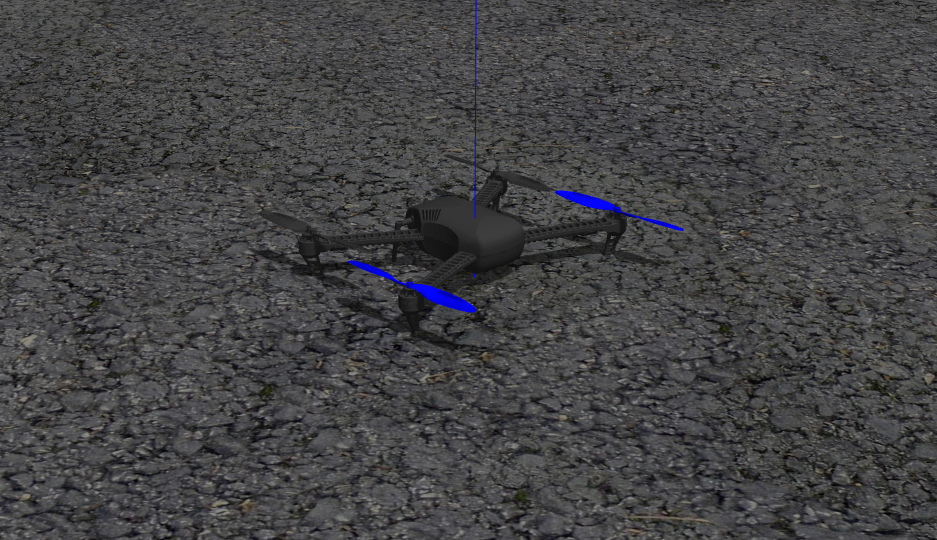
\includegraphics[height=4cm]{imagenes/cap4/1_px4_drone_gz.png}
	\end{center}
	\caption[3DR Iris simulado]{3DR Iris simulado}
	\label{fig:3dr_iris}
\end{figure}

\subsection{Teleoperador}
\label{subsec:teleoperador}

Ya propiamente hablando de resolver el problema planteado, la primera aproximación propuesta fue hacer una interfaz gráfica simple, que permitiera enviar órdenes a la aeronave.\\

Para ello, inicialmente se debía conseguir enviar mensajes de forma programática. Por tanto, se diseñó un \textbf{script controlador} encargado de la comunicación directa con el \textbf{controlador de la aeronave}, para enviar y recibir diversos datos vía MAVROS. De igual modo, se debían satisfacer una serie de requisitos que aseguraran el correcto funcionamiento del sistema:

\begin{enumerate}
	\item La comunicación debe darse a \textbf{más de 2Hz}, para evitar cambios indeseados en el funcionamiento interno del controlador PX4 (de la aeronave).

	\item Antes de realizar cualquier comunicación, \textbf{debe asegurarse que el estado es \emph{``connected''}}, lo que significa que el dron esta armado y en modo \emph{OFFBOARD} (nuestra aeronave posee 7 modos distintos, \emph{HOLD}, que mantiene la posición, \emph{RETURN}, que vuelve al punto de despegue, \emph{MISSION}, que permite cargar rutas programadas con anterioridad, \emph{TAKEOFF}, habilita el despegue, \emph{LAND}, habilita el aterrizaje, \emph{FOLLOW ME}, que permite seguir objetivos, y \emph{OFFBOARD}, que permite comandar al dron sin necesidad de GPS, lo que es útil de cara al desarrollo de aplicaciones robóticas) \cite{flight-modes}.
	
    \item Una vez esta conectado, se deben \textbf{enviar datos} (velocidades en nuestro caso) al controlador PX4, con el fin de \textbf{evitar el cierre de la conexión}. Estos datos carecen de utilidad más que la de asegurar dicha conectividad.
    
    \item Por último, y antes de enviar cualquier posición, velocidad o comando (distintos modos de actuación), se debe comprobar siempre que el \textbf{modo activo} es \emph{OFFBOARD} y que el dron esta \textbf{armado} (listo para volar). En caso contrario, se debe solicitar al controlador, mediante servicios, dichas especificaciones.
\end{enumerate}

Por tanto, con todo esto funcionando de forma correcta, la manera de generar comportamientos en el dron en sí, es mediante \emph{topics}. Concretamente, los que genera MAVROS automáticamente cuando se lanza todo el sistema. Tal y como se comentó en apartados previos, estos \emph{topics} sólo admiten mensajes \ac{ROS}, lo que encapsula el mensaje real transmitido al controlador PX4, que solo es compatible con MAVLINK.\\

En nuestro caso, enviaremos posiciones (PoseStamped), velocidades (Twist) y comandos (sevicios formados por mensajes personalizados, creados por MAVROS, con formato \ac{ROS}). Esto, nos permitirá conectar el resto de aplicaciones con el script controlador, mediante \emph{topics} comunes, de forma que se encargue de enviar la acción final al dron, mientras el resto de scripts se encarguen de resolver otras tareas.\\

De este modo, inicia el desarrollo propiamente dicho del \textbf{teleoperador}. El teleoperador, se diseñó con el fin de generar comportamientos que se usarían en las fases finales del \ac{TFG}. Sin embargo, en la primera versión, tan solo se buscó construir una interfaz gráfica sencilla, capaz de enviar ordenes usando \ac{ROS} que, en última instancia, llegasen al dron y produjesen diversos comportamientos, tales como \textbf{moverse y girar}, a través de sliders.\\

\begin{figure} [H]
	\begin{center}
	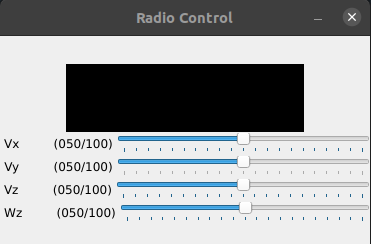
\includegraphics[height=4.5cm]{imagenes/cap4/2_axes_rc.png}
	\end{center}
	\caption[Primera versión del teleoperador]{Primera versión del teleoperador}
	\label{fig:teleoperador_v1}
\end{figure}

En el siguente paso, se buscó programar \textbf{comportamientos predefinidos}, es decir, acciones predeterminadas tales como desplazarse distancias concretas en ciertas direcciones, o girar un número específico de grados en un sentido u otro. Para ello, se diseñó una ampliación sobre la interfaz anterior, en la que se añadió un \textbf{botón por cada acción} concreta desarrollada, además de una \textbf{imagen de la cámara frontal} en directo. Es importante destacar la acción de moverse de distancias específicas, ya que se empleará en los algoritmos posteriores.\\

Finalmente, y continuando con lo anterior, se intentó afinar el comportamiento de las acciones predefinidas, para hacer que el dron se desplazase de celda en celda, concretamente de \textbf{centro en centro}. La idea es que, el dron solo tomará medidas de la señal en posiciones concretas y no en movimiento. Además, se agregaron \textbf{marcadores en \emph{rviz}}, para determinar las celdas visitadas (con colores aleatorios), junto con otro marcador que muestra la trayectoria que sigue la aeronave.\\

\begin{figure} [H]
	\begin{center}
	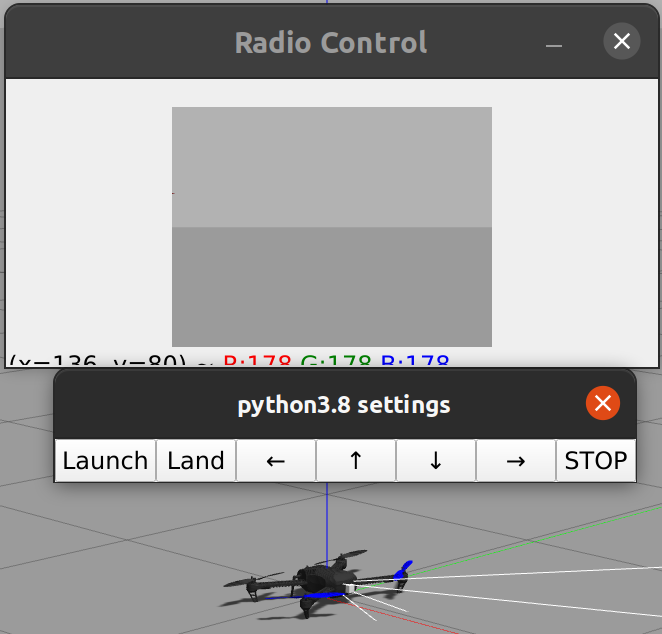
\includegraphics[height=8cm]{imagenes/cap4/3_c2c_gui.png}
	\end{center}
	\caption[Versión final del teleoperador]{Versión final del teleoperador}
	\label{fig:teleoperador_end}
\end{figure}

\newpage
A continuación, se muestra el \emph{``main''} de la aplicación mencionada:\\

\begin{code}[H]
\begin{lstlisting}[language=Python]
if __name__ == '__main__':
    try:
        rospy.init_node(NODENAME, anonymous=True)

        # Msgs
        ## Subscribers
        image_sub = rospy.Subscriber(IMAGE_TOPIC, Image, callback = image_cb)
        current_pos_sub = rospy.Subscriber(LOCAL_POSE_TOPIC, PoseStamped, callback = current_pos_cb)

        ## Publishers
        pos_pub = rospy.Publisher(RADIO_CONTROL_POS_TOPIC, PoseStamped, queue_size=10)
        cmd_pub = rospy.Publisher(RADIO_CONTROL_CMD_TOPIC, Px4Cmd, queue_size=10)

        # -- OPENCV -- #
        cv2.namedWindow(WINDOWNAME)

        # Buttons
        cv2.createButton('Launch', launch_button, None, cv2.QT_PUSH_BUTTON, 1)
        cv2.createButton('Land', land_button, None, cv2.QT_PUSH_BUTTON, 1)
        cv2.createButton('←', left_button, None, cv2.QT_PUSH_BUTTON, 1)
        cv2.createButton('↑', front_button, None, cv2.QT_PUSH_BUTTON, 1)
        cv2.createButton('↓', back_button, None, cv2.QT_PUSH_BUTTON, 1)
        cv2.createButton('→', right_button, None, cv2.QT_PUSH_BUTTON, 1)
        cv2.createButton('STOP', stop_button, None, cv2.QT_PUSH_BUTTON, 1)

        cv2.waitKey(0)
        cv2.destroyAllWindows()
    except rospy.ROSInterruptException:
        pass
\end{lstlisting}
\caption[Main de center to center app]{Main de center to center app}
\label{cod:c2c_app}
\end{code}

Donde, tras inicializar el nodo \ac{ROS}, se definen por un lado los \textbf{suscriptores}, encargados de recibir los datos de la cámara y la posición del dron (usando MAVROS), los \textbf{publicadores}, cuya función es enviar posiciones y/o comandos al script controlador, y por último la \textbf{interfaz gráfica} diseñada con \textbf{OpenCV}, donde se define la ventana y los botones con las diversas acciones predefinidas \footnote{Código completo en \url{https://github.com/RoboticsLabURJC/2022-tfg-cristian-sanchez/blob/main/src/teleop/scripts/c2c_control.py}}.\\

\section{Señales}
\label{sec:signals}

Continuando con el proyecto, entramos en el segundo gran bloque, las señales \ac{RF}. Este apartado, fue especialmente relevante, ya que nos permitió desarrollar una aplicación reactiva, con la meta de generar entornos sobre los que probar soluciones robóticas.\\

Pero, antes de entrar en detalle, conviene familiarizarse con algunos conceptos básicos sobre el procesamiento de señales:

\begin{enumerate}
	\item \textbf{Señal}:
	
    \item \textbf{Dominio temporal}:
    
    \item \textbf{Dominio de la señal}:
    
    \item \textbf{ADC}:
    
    \item \textbf{RSSI}:
    
    \item \textbf{SNR}:

    \item \textbf{Frecuencia}:
    
    \item \textbf{TX}:
    
    \item \textbf{RX}:
\end{enumerate}

Definidos estos términos, nuestro objetivo fue obtener un modelo capaz de calcular la \textbf{propagación de la señal}, es decir, -----.\\

\subsection{Aproximación de Friis}
\label{subsec:friis}

Por ello, se optó por emplear la aproximación de Friis, que nos proporciona una sencilla fórmula sobre la cual modelizar nuestro problema.\\

(insertar fórmula)

Donde cada término significa lo siguiente:

\begin{enumerate}
    \item \textbf{Ganancias}:
    
    \item \textbf{Valor lambda}:
    
    \item \textbf{Distancia (d)}:
    
    \item \textbf{Factor L}: (Insertar tabla)
\end{enumerate}

Además, empleando este método, podemos modelizar las \textbf{pérdidas de una señal} estimadas durante su propagación, a través de la siguiente ecuación:\\

(insertar ecuación path loss)\\

Sin embargo, para nuestro caso no es relevante (aunque se añadió al módulo).\\

\subsection{Módulo python de Friis}
\label{subsec:friis-module}

ToDo...

\subsection{Aplicación de Friis}
\label{subsec:friis-app}

ToDo...